% ------------------------------------------------------------------------------
% In the design section a general overview about the system to be implemented is
% shown. All the hardware, software, communications and other topics are
% evaluated and selected.
% ------------------------------------------------------------------------------

\opt{never}{\addbibresource{03-tail/bibliography.bib}} % to make citation found in most IDE

\chapter{Design}
\label{chap:design}

% -- Your text goes here --
The design shows an overview of the different parts of the reference architecture. It describes the idea behind the structure of the \gls{cloud_infrastructure} with the integration of several embedded systems. The general operation of each of the applications included in this architecture is also described.

\minitoc
\newpage

% ------------------------------------------------------------------------------
\section{Reference architecture}

% -- Your text goes here --
The reference architecture is divided into two parts: the first concerns embedded systems based on \gls{arm} architectures and certified \nameref{sec:arm_systemready} with a Linux operating system, while the second relates to the \gls{cloud} and is hosted by the \gls{aws} provider. An overview is clearly shown in figure \ref{fig:RefArch_Overview}.
\begin{center}
    \begingroup
    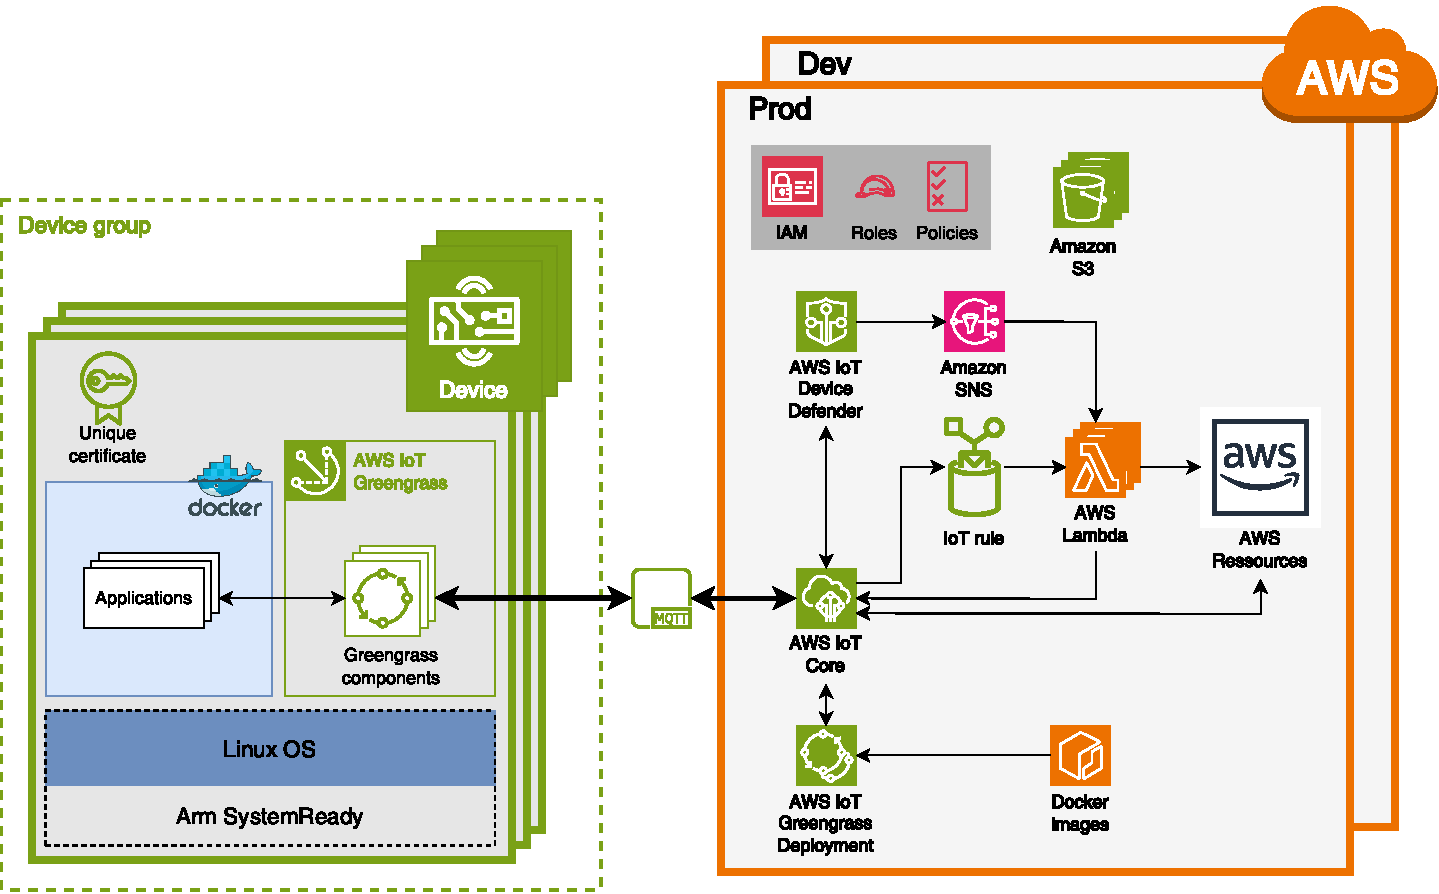
\includegraphics[width=1\columnwidth]{design/RefArch_Overview.pdf}
    \captionof{figure}{Reference architecture overview}
    \label{fig:RefArch_Overview}
    \endgroup
\end{center}

\subsection{\Gls{cloud_infrastructure}}
In the \gls{cloud}, two distinct infrastructures are presented. The first infrastructure is dedicated to development, enabling all kinds of operations to be tested. The second infrastructure is the production infrastructure, encompassing the final product intended for customers. Each infrastructure uses different \gls{aws} services.

The central service managing the \acrshort{iot} is \gls{aws} \acrshort{iot} Core, which exchanges data with all connected devices. Its preferred communication protocol is MQTT. Provisioned devices are registered in a specific group within this service. Only authorised devices are provisioned. \gls{aws} \acrshort{iot} Greengrass Deployment handles the deployment of new Greengrass components or updates to a group of devices. A component, in the context of \gls{aws} \acrshort{iot} Greengrass, is a unit of deployment and execution that encapsulates code, dependencies and resources, making it easy to deploy, manage and update \acrshort{iot} applications. In this architecture, Docker components are used, encapsulating Docker containers to offer greater flexibility in software deployment. Docker images are stored in the Amazon Elastic Container Registry (ECR). Another service, \gls{aws} \acrshort{iot} Device Defender, checks daily whether a certificate is about to expire, as each device has a unique certificate enabling a secure connection. If a certificate expires within 30 days, it is replaced by a new one. Other Lambda functions, triggered by rules, can enrich the architecture, as can other \gls{aws} resources, depending on the needs of each developer. Storage spaces such as Amazon S3 are used to save the state of the infrastructure, configuration files and \acrshort{os} images. The configuration files contain a list of the serial numbers of all the \acrshort{iot} devices authorised to be provisioned. If a device is not listed and attempts to be provisioned, access will be denied. If a device is already provisioned and its serial number is removed from the list, its access will be withdrawn and it will be deleted from the \gls{cloud}. The IAM service is there to assign roles and policies, limiting authorised actions on resources to the strict minimum.

\subsection{Embedded systems integration}
Embedded systems must be based on \gls{arm} architecture and be \nameref{sec:arm_systemready} certified. The devices are flashed with a custom Linux \acrshort{os} image. On first boot, two software programs are installed : Docker Engine for running Docker containers, and \gls{aws} \acrshort{iot} Greengrass Core for \gls{provisioning}, communicating with \gls{aws} \acrshort{iot} Core and managing Greengrass components. This software provisions the device by exchanging the claim certificate with a unique certificate, securing the connection of the device, which is then registered in the device group. Deployment of Greengrass components from the \gls{cloud} to devices is automated when a new device is associated or a new version of a component becomes available. Applications are contained in Docker containers to ensure optimum portability.